\chapter{TÌNH HÌNH THỰC TẬP VÀ KẾT QUẢ DỰ ÁN RAREPROTSELECT}
\label{chap:tinh_hinh_du_an}

Chương này trình bày toàn diện nội dung công việc chuyên môn mà tôi được giao thực hiện tại ORLab: từ việc bóc tách bài toán chọn tập protein đại diện trong tin sinh học, xây dựng mô hình toán học tối ưu hóa submodular có trọng số phạt quy mô nhóm, tích hợp mô hình ngôn ngữ protein ESM-2, đến việc đo đạc và phân tích 6 kịch bản thực nghiệm đối chuẩn trên tập dữ liệu MEROPS A1A.

\section{Tổng quan về đề tài nghiên cứu RareProtSelect}
\label{sec:tong_quan_du_an}

Với sự phát triển mạnh mẽ của sinh học phân tử và tin sinh học, các cơ sở dữ liệu sinh học đang chứng kiến sự bùng nổ dữ liệu với hàng trăm triệu chuỗi protein. Việc phân tích hoặc mô phỏng phân tử trên toàn bộ cơ sở dữ liệu đòi hỏi chi phí tính toán cực kỳ lớn. Do đó, bài toán lựa chọn một tập con đại diện gồm $k$ chuỗi, với $k \ll |V|$, nhưng vẫn phản ánh tối đa độ đa dạng sinh học và các đặc tính chức năng của toàn thể siêu họ protein trở thành một thách thức nền tảng trong tin sinh học tính toán~\cite{nguyen2025}.

Tuy nhiên, các họ protein trong tự nhiên luôn chịu sự chi phối của phân bố đuôi dài Long-Tail do quy luật tiến hóa sinh học. Điển hình như Family Peptidase A1 thuộc Clan AA trong cơ sở dữ liệu MEROPS~\cite{merops}: sau khi sàng lọc và thẩm định dữ liệu thu được $4.120$ chuỗi protein đã qua kiểm soát chất lượng thuộc $115$ Subfamily chính thức. Phân bố số lượng chuỗi giữa các nhóm có mức độ mất cân bằng cực đoan lên tới $\frac{n_{\max}}{n_{\min}} = \frac{329}{1} = 329{,}0$ lần, từ Subfamily lớn nhất A01.009 gồm $329$ chuỗi đến $8$ Subfamily đơn độc chỉ có đúng $1$ chuỗi thành viên.

Các phương pháp truyền thống hiện có, bao gồm phân cụm chuỗi CD-HIT~\cite{cdhit}, MMseqs2~\cite{mmseqs2}, và bài báo nền tảng sử dụng hàm submodular Facility Location tiêu chuẩn~\cite{nguyen2025} mắc phải một điểm mù phương pháp luận trọng yếu: mô hình tối ưu hóa không trọng số luôn ưu tiên phân bổ đại diện vào các Subfamily đông chuỗi nhằm tối đa hóa tổng độ tương đồng toàn cục. Kết quả là tại các mức ngân sách đại diện nhỏ và trung bình từ $k = 11$ đến $k = 115$, gần như toàn bộ các Subfamily hiếm bị bỏ sót, chỉ đạt tối đa $2{,}22\%$ Rare Sensitivity tại $k = 115$, gây mất mát nghiêm trọng các biến dị tiến hóa và cấu trúc phân tử quý hiếm.

\section{Mô hình hóa toán học và phương pháp đề xuất}
\label{sec:phuong_phap_mo_hinh_hoa}

Để giảm thiểu tối đa sự thiên lệch quy mô mẫu, đề tài RareProtSelect đề xuất mô hình toán học tối ưu hóa submodular Facility Location~\cite{wei2015} có trọng số phạt quy mô nhóm kết hợp biểu diễn không gian tương đồng hai chiều.

\subsection{Hàm mục tiêu Facility Location có trọng số phạt quy mô nhóm}
Xét tập toàn thể gồm $|V| = N$ chuỗi protein $V = \{1, 2, \dots, N\}$ được phân chia thành $G$ Subfamily chính thức $V = \bigcup_{g=1}^G V_g$. Dựa trên nguyên lý tái cân bằng phân bố đuôi dài~\cite{cui2019}, với mỗi chuỗi $v \in V_g$, trọng số tối ưu hóa được xác định theo công thức:
\begin{equation}
    w_v^{(\alpha)} = (n_g)^{-\alpha}
    \label{eq:sample_weight}
\end{equation}
trong đó $n_g = |V_g|$ là quy mô số lượng chuỗi của Subfamily $g$, và $\alpha \in [0{,}0; 1{,}0]$ là hệ số tái cân bằng mức ưu tiên tối ưu hóa.
\begin{itemize}[noitemsep,topsep=2pt]
    \item Khi $\alpha = 0{,}0$: mô hình trở về hàm Facility Location truyền thống của bài báo nền~\cite{nguyen2025}, nơi mọi chuỗi có trọng số bằng nhau, với $w_v = 1$.
    \item Khi $\alpha = 0{,}50$: trọng số cân bằng theo căn bậc hai, phân bổ sự quan tâm hài hòa giữa độ bao phủ tổng thể và nhóm hiếm.
    \item Khi $\alpha = 1{,}0$: trọng số tỷ lệ nghịch hoàn toàn với quy mô nhóm, bảo đảm mỗi Subfamily có tổng trọng số đóng góp danh nghĩa ngang nhau trong hàm mục tiêu.
\end{itemize}

Hàm mục tiêu lựa chọn tập đại diện $S \subseteq V$ với ngân sách $|S| \le k$ được định nghĩa qua công thức~\eqref{eq:weighted_facility_location}:
\begin{equation}
    F_\alpha(S) = \sum_{v \in V} w_v^{(\alpha)} \max_{s \in S} \mathbf{S}(v, s)
    \label{eq:weighted_facility_location}
\end{equation}
trong đó $\mathbf{S}(v, s) \in [0{,}0; 1{,}0]$ là giá trị tương đồng giữa hai chuỗi protein $v$ và $s$.

Hàm $F_\alpha(S)$ được chứng minh toán học giải tích là một hàm đơn điệu không giảm và submodular. Do đó, giải thuật tham lam Greedy được bảo đảm về mặt lý thuyết đạt tỷ lệ xấp xỉ tối thiểu bằng $(1 - 1/e) \approx 63{,}2\%$ so với nghiệm tối ưu toàn cục theo định lý Nemhauser~\cite{nemhauser1978} nổi tiếng.

\subsection{Giải thuật Pruned Greedy 90\% trên GPU và cơ chế tổng hợp thứ hạng toàn cục}
Trong bài báo nền~\cite{nguyen2025}, kịch bản Standard Greedy đánh giá toàn bộ ứng viên ở mỗi bước lặp. Dù giải thuật Lazy Greedy~\cite{minoux1978} dùng hàng đợi Max-Heap giúp giảm số lần gọi hàm mục tiêu, việc xử lý ma trận lớn trên CPU vẫn tốn kém. Do đó, đề tài cài đặt dạng vector hóa của giải thuật tham lam cắt tỉa Pruned Greedy 90\%~\cite{nguyen2025} tăng tốc trên môi trường tính toán GPU PyTorch CUDA.

Giải thuật duy trì một vector bao phủ lũy tích $\mathbf{coverage} \in [0, 1]^N$ với phần tử $\mathbf{coverage}_v = \max_{s \in S} \mathbf{S}(s, v)$ biểu diễn mức độ tương đồng cực đại hiện tại của chuỗi $v$ đối với tập đại diện đã chọn $S$. Tại mỗi bước lặp, độ tăng cận biên của ứng viên $u \in V \setminus S$ được tính toán song song qua phép nhân ma trận trên GPU:
\begin{equation}
    \Delta(u \mid S) = \sum_{v \in V} w_v^{(\alpha)} \max\bigl(0, \, \mathbf{S}(u, v) - \mathbf{coverage}_v\bigr)
    \label{eq:marginal_gain_gpu}
\end{equation}
Quy tắc cắt tỉa cứng với ngưỡng $\theta = 0{,}90$ kế thừa từ bài báo nền~\cite{nguyen2025}: khi chuỗi $v$ đạt độ bao phủ $\mathbf{coverage}_v \ge 0{,}90$, đóng góp cận biên của các ứng viên có độ tương đồng cao với $v$ triệt tiêu về $0$, loại bỏ việc chọn đại diện dư thừa trong cùng Subfamily.

Tuy nhiên, trong các họ protein có nhiều chuỗi có độ tương đồng giống hệt nhau, hiện tượng các ứng viên có cùng độ tăng cận biên $\Delta(u_1 \mid S) = \Delta(u_2 \mid S)$ dẫn đến sự phụ thuộc vào thứ tự duyệt mảng. Nhằm loại bỏ thiên lệch này, đề tài áp dụng cơ chế tổng hợp thứ hạng toàn cục qua $M = 1.000$ vòng xáo trộn ngẫu nhiên. Sau $1.000$ lần chạy độc lập, giải thuật tổng hợp tần suất $\text{Count}[v]$ và tổng thứ hạng $\text{RankSum}[v]$ của mỗi chuỗi để xác lập danh sách xếp hạng tổng hợp $S_{\text{aggregate}}$: chuỗi có tần suất xuất hiện cao hơn được xếp trước; trong trường hợp có cùng tần suất xuất hiện, quy tắc phân xử đồng hạng sẽ ưu tiên chuỗi có tổng thứ hạng nhỏ hơn, tức được giải thuật lựa chọn ở các bước lặp sớm hơn.

\subsection{Không gian biểu diễn tương đồng và kỹ thuật khử co cụm vector}
Đề tài khai thác và đối sánh hai không gian biểu diễn chuỗi protein:
\begin{enumerate}[noitemsep,topsep=2pt]
    \item \textbf{Không gian tương đồng gióng hàng cục bộ Live BLASTp $\mathbf{S}_{\text{BLAST}}$}: Ma trận đối soát chuỗi dựa trên thuật toán BLASTp truyền thống~\cite{blast} cùng bộ công cụ BLAST+ cải tiến~\cite{camacho2009}, phản ánh trực tiếp tỷ lệ nhận dạng axit amin bảo tồn qua tiến hóa.
    \item \textbf{Không gian vector nhúng ngữ nghĩa PLM ESM-2 $\mathbf{S}_{\text{ESM}}$}: Trích xuất vector đặc trưng $\mathbf{z}_v \in \mathbb{R}^{480}$ từ tầng ẩn cuối cùng của mô hình ngôn ngữ protein ESM-2 checkpoint 35M~\cite{esm2}.
\end{enumerate}

Để khắc phục hiện tượng co cụm vector Anisotropy - hiện tượng phổ biến trong các mô hình Transformer khiến các vector nhúng bị dồn về một nón hẹp dẫn tới độ tương đồng cosine luôn ở mức cao ảo~\cite{ethayarajh2019} - đề tài áp dụng kỹ thuật dịch tâm Mean-Centering:
\begin{equation}
    \tilde{\mathbf{z}}_v = \mathbf{z}_v - \frac{1}{|V|} \sum_{u \in V} \mathbf{z}_u
    \label{eq:mean_centering}
\end{equation}
Ma trận tương đồng kết hợp được định nghĩa qua tham số điều hòa $\beta \in [0{,}0; 1{,}0]$:
\begin{equation}
    \mathbf{S}_{\text{combined}} = (1 - \beta) \mathbf{S}_{\text{BLAST}} + \beta \mathbf{S}_{\text{ESM}}
    \label{eq:combined_similarity}
\end{equation}

\section{Kết quả thực nghiệm và phân tích định lượng}
\label{sec:ket_qua_thuc_nghiem}

Nhằm làm sáng tỏ cơ chế đánh đổi giữa năng lực bao phủ toàn thể và khả năng bảo tồn tính đại diện của các Subfamily hiếm, bảng~\ref{tab:exp2_pareto_milestones} đối chuẩn các chỉ số thực nghiệm giữa mô hình hàm mục tiêu cơ sở không trọng số ứng với $\alpha = 0{,}00$, kế thừa từ mô hình của \cite{nguyen2025}, và các cấu hình trọng số của RareProtSelect tại hai mốc ngân sách $k = 11$ và $k = 115$ trên tập MEROPS A1A.

\begin{table}[htbp!]
    \centering
    \caption{Đối chuẩn các chỉ số thực nghiệm giữa mô hình cơ sở không trọng số ứng với $\alpha = 0{,}00$ và các cấu hình trọng số RareProtSelect tại các mức ngân sách $k = 11$ và $k = 115$ trên tập MEROPS A1A.}
    \label{tab:exp2_pareto_milestones}
    \vspace{2pt}
    \renewcommand{\arraystretch}{0.92}
    \begin{tabularx}{\textwidth}{L{3.5cm} c c >{\centering\arraybackslash}p{2.2cm} >{\centering\arraybackslash}p{2.2cm} >{\centering\arraybackslash}X}
        \toprule
        \textbf{Phương pháp} & \textbf{Hệ số $\alpha$} & \textbf{Ngân sách $k$} & \textbf{Overall Sens, \%} & \textbf{Rare Sens, \%} & \textbf{Zero-Sensitivity Count} \\
        \midrule
        Mô hình cơ sở~\cite{nguyen2025} & $0{,}00$ & $11$ & $38{,}06$ & $0{,}00$ & $105$ \\
        RareProtSelect & $0{,}50$ & $11$ & $32{,}60$ & $0{,}00$ & $104$ \\
        RareProtSelect & $1{,}00$ & $11$ & $26{,}07$ & $4{,}44$ & $104$ \\
        \midrule
        Mô hình cơ sở~\cite{nguyen2025} & $0{,}00$ & $115$ & $93{,}57$ & $2{,}22$ & $58$ \\
        RareProtSelect & $0{,}50$ & $115$ & $94{,}13$ & $59{,}11$ & $23$ \\
        RareProtSelect & $1{,}00$ & $115$ & $79{,}08$ & $91{,}11$ & $18$ \\
        \bottomrule
    \end{tabularx}
\end{table}

Số liệu trích xuất nguyên văn từ tệp kết quả thực nghiệm tại bảng~\ref{tab:exp2_pareto_milestones} làm sáng tỏ các điểm mốc phương pháp luận trọng yếu:
\begin{enumerate}[noitemsep,topsep=2pt]
    \item Tại ngân sách nhỏ $k = 11$ chuỗi đại diện: mô hình không trọng số cơ sở với $\alpha = 0{,}00$ đạt $38{,}06\%$ Overall Sensitivity nhưng chưa lựa chọn được chuỗi đại diện nào từ $45$ Subfamily hiếm, tương ứng $0{,}00\%$ Rare Sensitivity, khiến $105$ trên $115$ Subfamily chưa có chuỗi nào được nhận diện. Khi tăng hệ số trọng số lên $\alpha = 1{,}00$, giải thuật bắt đầu ưu tiên lựa chọn đại diện của nhóm hiếm, đạt mức độ nhạy vĩ mô trung bình $4{,}44\%$ trên $45$ Subfamily hiếm ngay tại mức ngân sách rất nhỏ.
    \item Tại ngân sách $k = 115$, tương ứng mỗi Subfamily có trung bình $1$ đại diện: mô hình không trọng số cơ sở chỉ đạt $2{,}22\%$ Rare Sensitivity và bỏ sót tới $58$ Subfamily (Zero-Sensitivity Count bằng $58$). Ngược lại, cấu hình trọng số $\alpha = 0{,}50$ xác lập điểm cân bằng tốt nhất trong ba cấu hình khảo sát: Overall Sensitivity đạt $94{,}13\%$, cao hơn $0{,}56$ điểm phần trăm so với mô hình cơ sở, đồng thời thước đo Rare Sensitivity tăng lên $59{,}11\%$ (với nhiều phân họ hiếm đạt độ bao phủ toàn diện $100\%$ và các phân họ còn lại được nhận diện một phần), cắt giảm số Subfamily chưa có đại diện từ $58$ xuống còn $23$. Khi đẩy trọng số lên $\alpha = 1{,}00$, Rare Sensitivity đạt tới $91{,}11\%$, nhưng Overall Sensitivity bị sụt giảm từ $93{,}57\%$ xuống $79{,}08\%$ (mất $14{,}49$ điểm phần trăm) để đổi lấy việc đưa Zero-Sensitivity Count xuống còn $18$.
\end{enumerate}

Như vậy, tại mốc ngân sách $k = 115$, cấu hình trọng số $\alpha = 0{,}50$ giải quyết hiệu quả sự đánh đổi đa mục tiêu: vừa bảo toàn độ bao phủ toàn thể, vừa cải thiện rõ rệt tính đại diện cho các Subfamily hiếm trên không gian tương đồng Live BLASTp (hình~\ref{fig:exp2_pareto}). Tuy nhiên, sự cải thiện này đi kèm sự đánh đổi ở ngân sách nhỏ: tại $k = 11$, $\alpha = 0{,}50$ giảm $5{,}46$ điểm phần trăm Overall Sensitivity mà chưa thể thu hồi phân họ hiếm nào, còn $\alpha = 1{,}00$ mất tới $11{,}99$ điểm phần trăm để đổi lấy $4{,}44\%$ Rare Sensitivity.

\begin{figure}[htbp!]
    \centering
    \vspace{-6pt}
    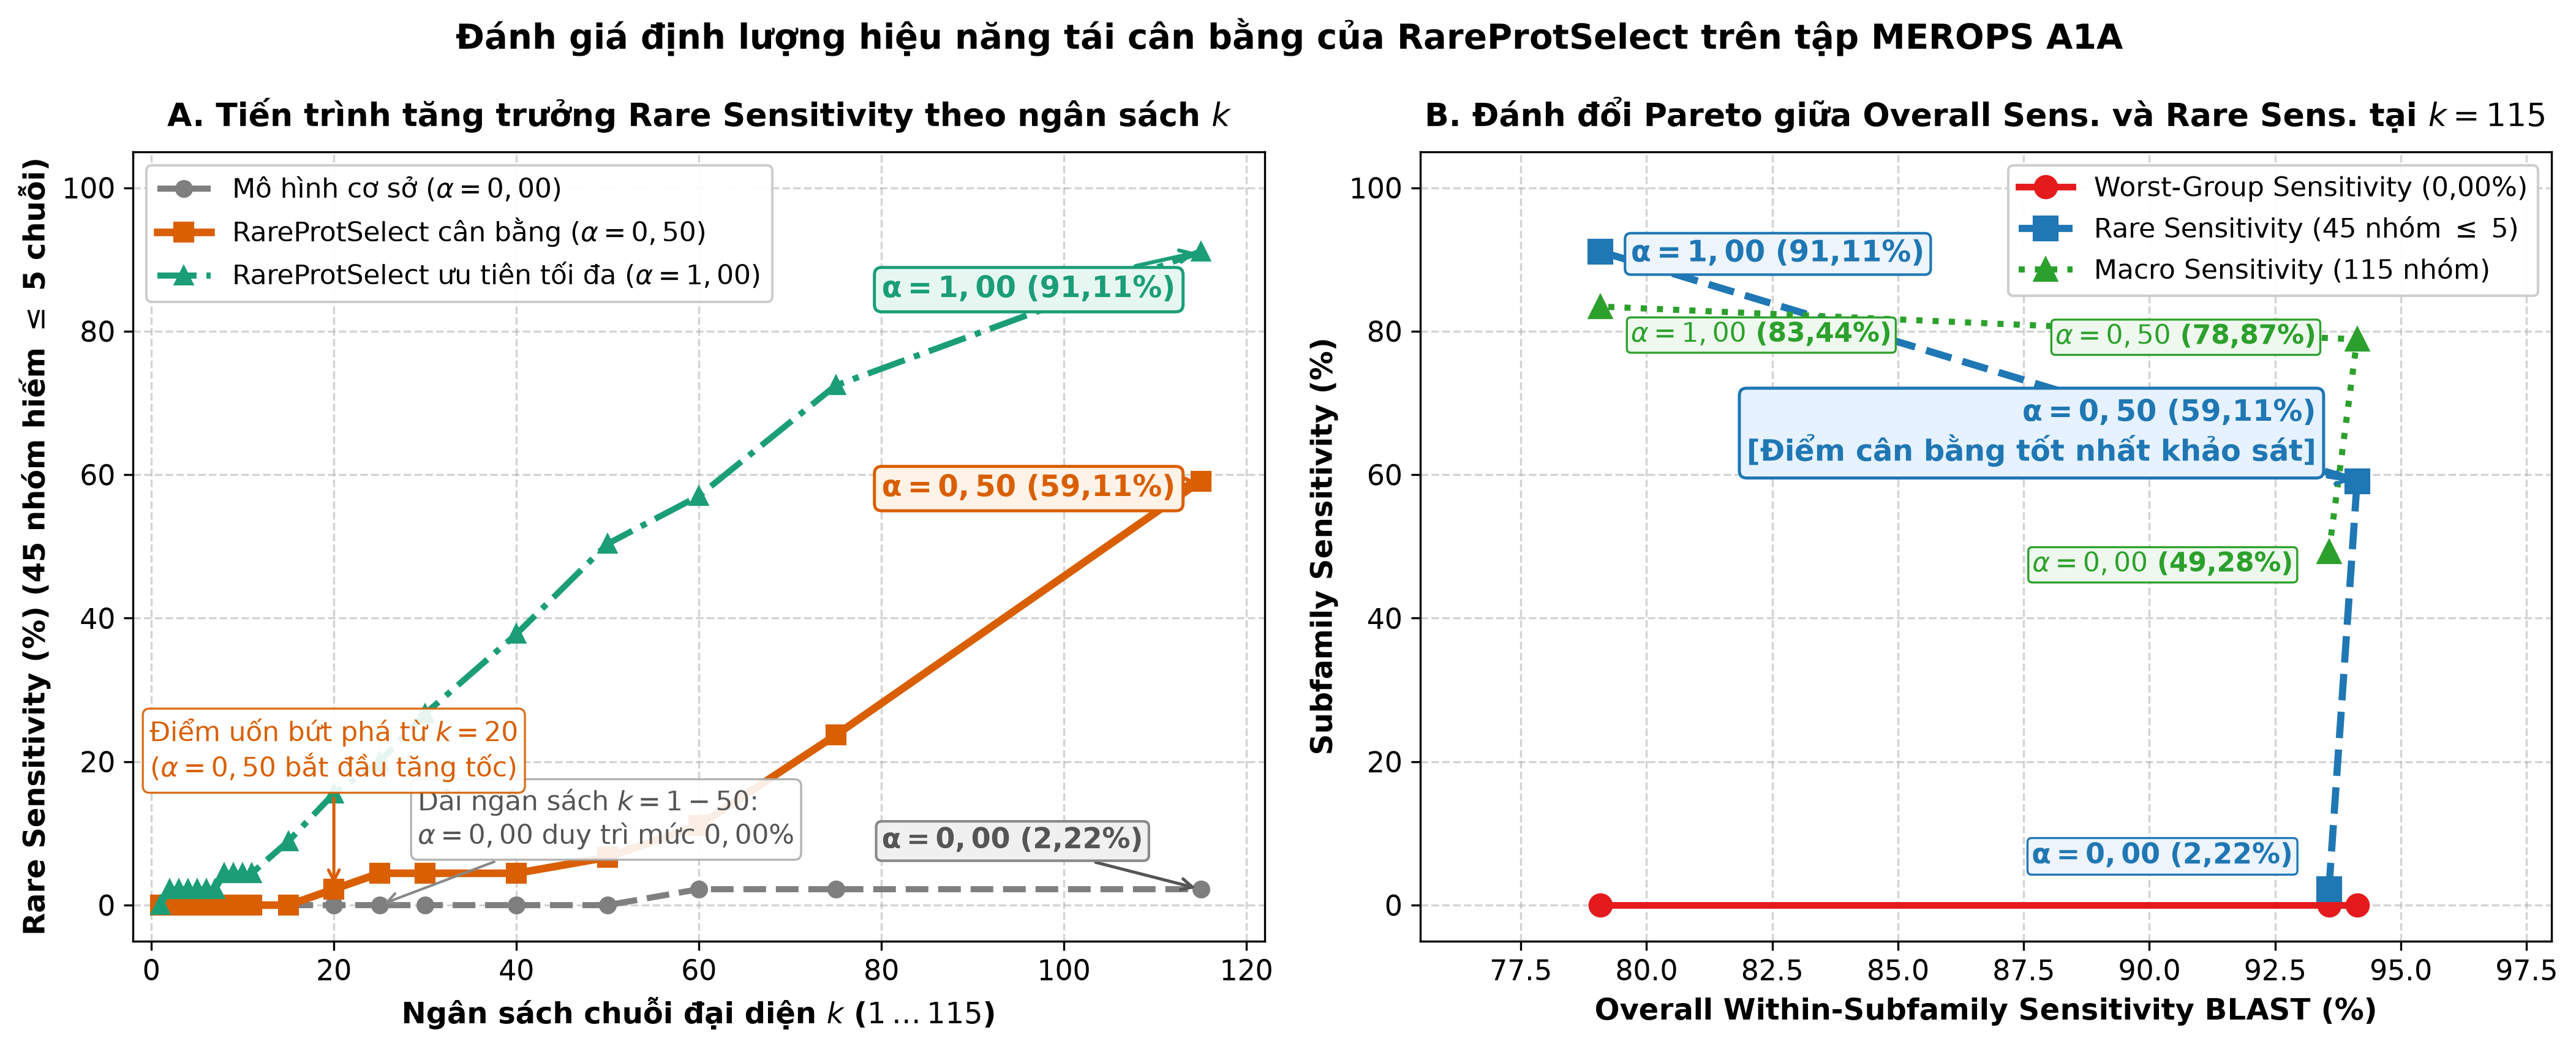
\includegraphics[width=0.68\textwidth]{Images/figures/exp2_pareto_tradeoff.png}
    \vspace{-6pt}
    \caption{Đánh giá hiệu năng của RareProtSelect trên tập MEROPS A1A: (A) Tiến trình Rare Sensitivity theo ngân sách $k \in [1, 115]$; (B) Đánh đổi Pareto giữa Overall Sensitivity và Subfamily Sensitivity tại $k = 115$.}
    \label{fig:exp2_pareto}
    \vspace{-6pt}
\end{figure}

Đồ thị tại hình~\ref{fig:exp2_pareto} phản ánh rõ nét hai góc nhìn phương pháp luận:
\begin{itemize}[noitemsep,topsep=1pt]
    \item \textbf{Tiến trình theo ngân sách (Hình~\ref{fig:exp2_pareto}A)}: mô hình cơ sở $\alpha = 0{,}00$ duy trì Rare Sensitivity xấp xỉ $0\%$ suốt dải $k = 1 - 50$ và chỉ đạt $2{,}22\%$ tại $k = 115$. Trong khi đó, RareProtSelect $\alpha = 0{,}50$ tăng tốc từ mốc $k = 20$ và đạt $59{,}11\%$ tại $k = 115$, còn $\alpha = 1{,}00$ đạt $91{,}11\%$.
    \item \textbf{Đánh đổi Pareto tại $k = 115$ (Hình~\ref{fig:exp2_pareto}B)}: Tại $k = 115$, cấu hình $\alpha = 0{,}50$ đạt giá trị cao hơn mô hình cơ sở $\alpha = 0{,}00$ trên cả ba chỉ số: Overall Sensitivity đạt $94{,}13\%$ so với $93{,}57\%$, Macro-Average Sensitivity đạt $78{,}87\%$ so với $49{,}28\%$ và Rare Sensitivity đạt $59{,}11\%$ so với $2{,}22\%$, xác lập điểm cân bằng tốt nhất trong ba cấu hình khảo sát.
\end{itemize}

\section{Kiến trúc kỹ thuật và công nghệ triển khai tại ORLab}
\label{sec:kien_truc_cong_nghe}

Hệ thống mã nguồn của đề tài được đóng gói chuẩn mực trong thư mục \textbf{RareProtSelect/}:
\begin{itemize}[noitemsep,topsep=0pt,partopsep=0pt]
    \item \textbf{Môi trường và trình quản lý gói}: Quản lý môi trường ảo độc lập qua công cụ uv trên nền Python 3.12, bảo đảm tốc độ cài đặt và tính tái lập chuẩn xác.
    \item \textbf{Tăng tốc tính toán phần cứng}: bộ xử lý AMD Ryzen 9 8940HX ($16$ nhân, $32$ luồng) kết hợp GPU NVIDIA RTX 5060 ($8\text{ GB}$ GDDR6, CUDA 13.0). Phép trích xuất embedding ESM-2 và tính toán ma trận thực thi trực tiếp trên GPU.
    \item \textbf{Cấu hình thí nghiệm tự động}: Sử dụng các tệp cấu hình YAML phân tách rõ ràng giữa tham số mô hình $\alpha, \beta, k$, đường dẫn dữ liệu và kịch bản thực nghiệm, phục vụ quy trình chạy hàng loạt ổn định.
\end{itemize}
